\documentclass[11pt]{article}
\usepackage[utf8]{inputenc}
\usepackage{amsmath,amssymb,amsthm}
\usepackage{graphicx}
\usepackage{hyperref}
\usepackage{algorithm}
\usepackage{algorithmic}
\usepackage{booktabs}
\usepackage{wrapfig}

\title{ *WIP* tatbot: Tattoo Robot}
\author{Hugo Ponte}
\date{\today}

\begin{document}
\maketitle

\begin{figure}[h]
    \centering
    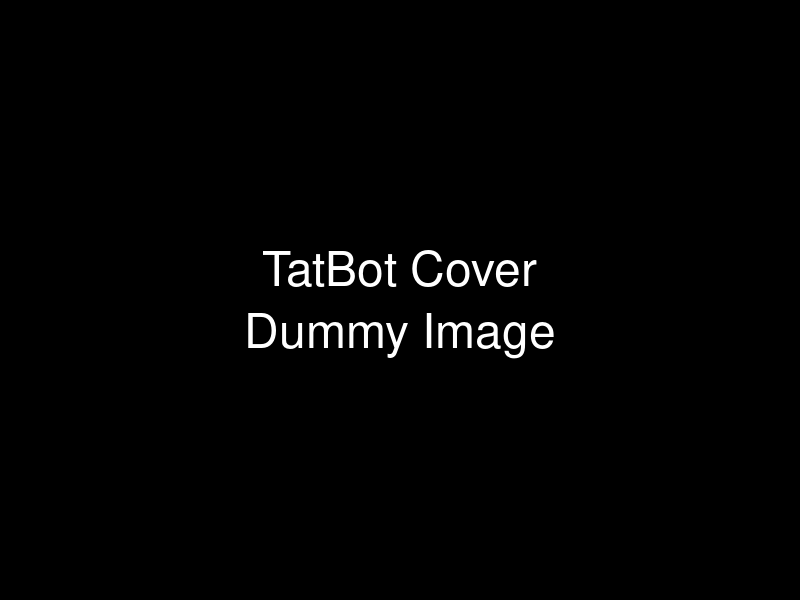
\includegraphics[width=0.8\textwidth]{figures/cover.png}
    \caption{(a) The tatbot system (hardware v0.2) (b) First human tattoo performed by the tatbot system. }
    \label{fig:cover}
\end{figure}


\begin{abstract}
*WIP* We present \textbf{tatbot}, an autonomous robotic system designed to perform tattoo artistry.
\end{abstract}

\pagebreak

\begin{figure}[h]
    \centering
    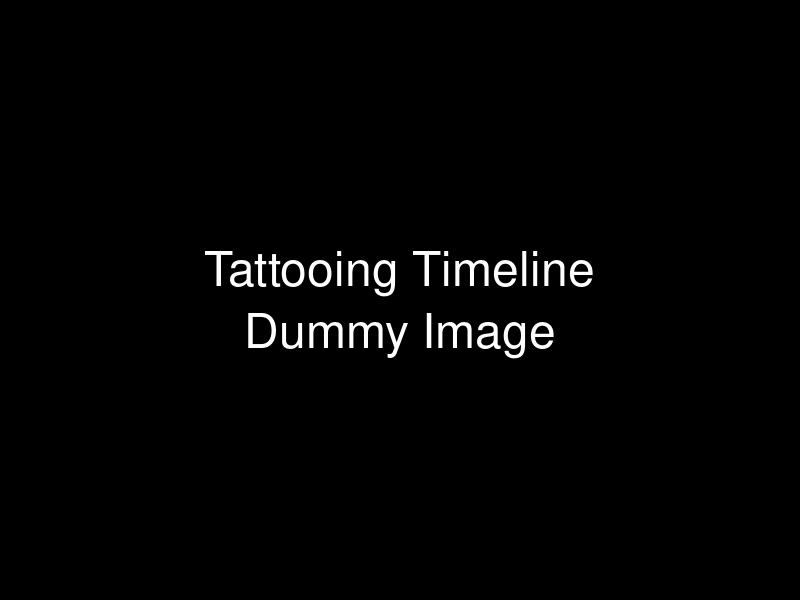
\includegraphics[width=0.8\textwidth]{figures/timeline.png}
    \caption{A history of tattoos.}
    \label{fig:timeline}
\end{figure}

\section{Background}

\subsection{History}

hupo

Tattoos are an ancient art form that predates recorded history.
Tattoos have been used as punishment, status symbols, and even therapeutic tools.
Ötzi, a frozen mummy found in the alps dated to 6272 BP, had tattoos on his arthritic joints \cite{deterwolf_worlds_oldest}.
The Yimkhiungs of Northern India perform ritualized tattooing on children as young as 5 yearls old \cite{kluger2015cultural}.
In ancient Mesopotamia, tattooing was used to mark slaves to punitively identify criminals \cite{hawken2022tattooing}.
Today tattoos have evolved and merged into a global art form that is practiced in every corner of the world.
Though some of the original symbology and purpose still remains, most modern tattoos are purely aesthetic.
In many cultures, tattoos have to be "earned". They might represent a rite of passage, family sigil, or national identy. There is still debate over cultural appropriation of tattoos.
Tattoo comes from a polynesian word \textit{tatau} which means \textit{to strike}, a reference to the traditional method of tattooing where needle penetration is achieved by striking with stick.
During the 18th and 19th centuries, the age of exploration introduced Polynesian tattoos to the west.
As a result, most modern languages now use the loanword tattoo to describe the art form over whatever traditional terminology may have existed.

\subsection{History}

grok4

Tattooing is one of the oldest forms of body modification, with evidence dating back to the Neolithic period. The earliest known tattoos belong to "Otzi the Iceman, a 5,300-year-old mummy discovered in the "Otztal Alps, featuring 61 carbon-based tattoos likely placed for therapeutic purposes on arthritic joints \cite{Samadelli2015,deterwolf_worlds_oldest}. Similar ancient tattoos have been identified on Egyptian mummies from around 2000 BCE, including figurative designs possibly linked to fertility and protection \cite{friedman2018natural}. In the Americas, the oldest tattoos appear on a Chinchorro mummy from Chile, dated to 2563--1972 BCE, consisting of dotted lines \cite{arrietamummies}. Across prehistoric and ancient societies, tattoos served diverse functions: medicinal and protective in Europe and Egypt; markers of social status, lineage, and rites of passage in Austronesian cultures like those in Polynesia and Micronesia \cite{kluger2015cultural}; and symbols of achievement or spiritual significance among indigenous groups in North America, such as the Osage and Haudenosaunee \cite{deterwolf2013drawing}.
In various ancient civilizations, tattooing also carried punitive connotations. In Mesopotamia, it was used to brand slaves and criminals \cite{hawken2022tattooing}, a practice echoed in Greco-Roman societies where tattoos stigmatized captives, deserters, and gladiators \cite{jones1987stigma}. Among the Thracians, however, tattoos signified nobility. In Asia, Chinese and Japanese tattoos evolved from spiritual markings to punitive brands during certain periods, influencing modern Yakuza traditions \cite{krutak2012tattooing}. Indigenous practices, such as the hand-tapped tattoos of Samoa (pe'a for men, malu for women), emphasized endurance and social hierarchy, while Inuit women used facial tattoos (kakiniit) to denote maturity and spiritual readiness \cite{johnston2017reawakening}.
The term tattoo'' derives from the Polynesian word \textit{tatau}, meaning to strike,'' referring to traditional tapping methods with bone tools. European contact during the Age of Exploration, notably Captain James Cook's voyages in the 18th century, introduced Polynesian tattooing to the West, leading to its adoption among sailors and eventual integration into global terminology \cite{friedman2014cook}. By the 19th century, tattoos spread through colonial encounters, often associated with marginal groups like convicts and military personnel.
In contemporary society, tattooing has transformed into a widespread art form practiced worldwide, blending traditional symbolism with aesthetic expression. While some cultures retain ``earned'' tattoos representing rites of passage or heritage---such as those among the Yimkhiung of Northern India, where children as young as five undergo ritual tattooing \cite{kluger2015cultural}---most modern tattoos are decorative. Debates persist over cultural appropriation, particularly of indigenous designs. The Tattoo Renaissance since the 1970s has mainstreamed the practice, driven by technological advancements like the electric tattoo machine (patented in 1891) and media exposure, with tattoos now symbolizing personal identity, reclamation, and artistic innovation \cite{schildkrout2004inscribing,roberts2012secret}.

\subsection{Biology}

\begin{wrapfigure}{l}{0.5\textwidth}
    \vspace{-20pt}
    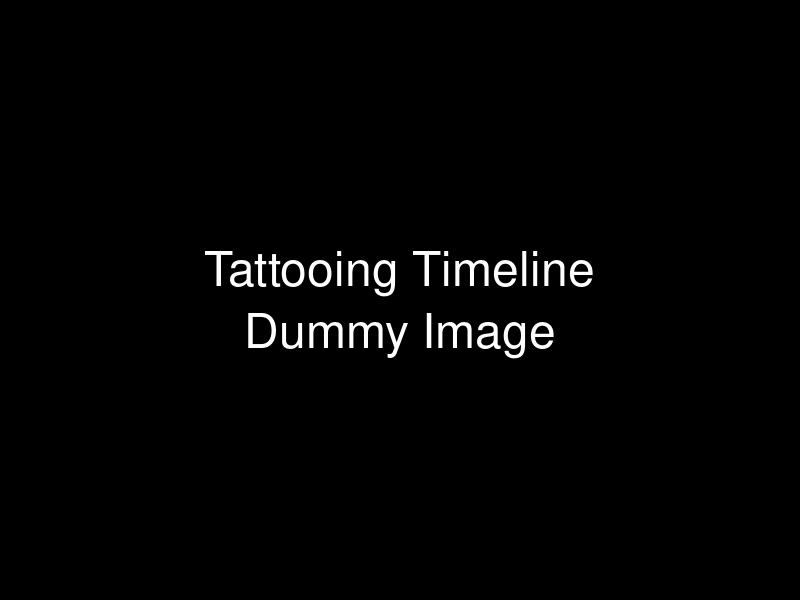
\includegraphics[width=\linewidth]{figures/timeline.png}
    \caption{A history of tattoos.}
    \label{fig:timeline_biology}
\end{wrapfigure}

The human skin is a complex organ, but it can roughly be divided into three layers:

\begin{itemize}
    \item Epidermis: outermost layer, 0.1 to 0.5mm thick, contains melanocytes, keratinocytes, and melanin.
    \item Dermis: middle layer, 1 to 4mm thick, contains blood vessels, nerves, and hair follicles.
    \item Subcutaneous tissue: innermost layer, 1 to 4mm thick, contains fat and connective tissue.
\end{itemize}

In a perfect tattoo, each needle puncture will deposit ink particles into the dermis.
Ink deposited in the epidermis will fade as the skin cells regenerate.
Ink deposited in the subcutaneous tissue will "blow out" as it diffuses outwards from the puncture site.
because tattoos penetrate the skin, they can be a vector for disease transmission.
medical grade equipment and sanitation protocols are required to prevent infection.

\begin{figure}[h]
    \centering
    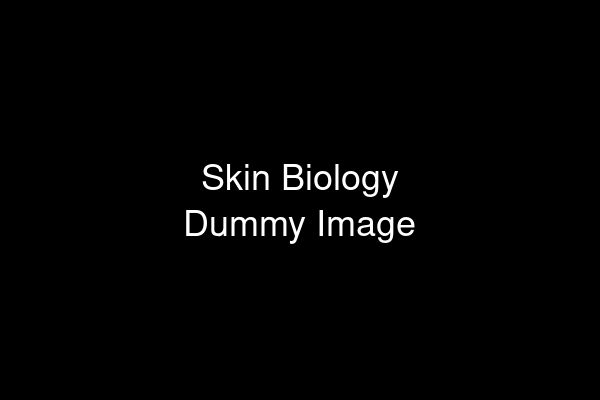
\includegraphics[width=0.8\textwidth]{figures/biology.png}
    \caption{A history of tattoos.}
    \label{fig:timeline}
\end{figure}

\pagebreak

\subsection{Technology}

Tattoo machines can be classified into two rough categories: rotary and coil.
rotary machines have become the standard for modern tattooing.
a wide variety of manufacturers compete to create the best wireless battery powered rotary machines.
voltage is modulated to control the speed of the motor, ranging from 3V to 12V.
needles are sold in pre-packaged cartridges, providing a convenient sterilized one-time use needle.
many cartridge types and vendors exist
needles are classified by their diameter, a grouping pattern, taper type, and length.
rotary machines use the rotational motion of a small electric motor to drive the up and down motion of the needle.
The distance the needle travels is called the \textit{stroke length}.

\begin{figure}[h]
    \centering
    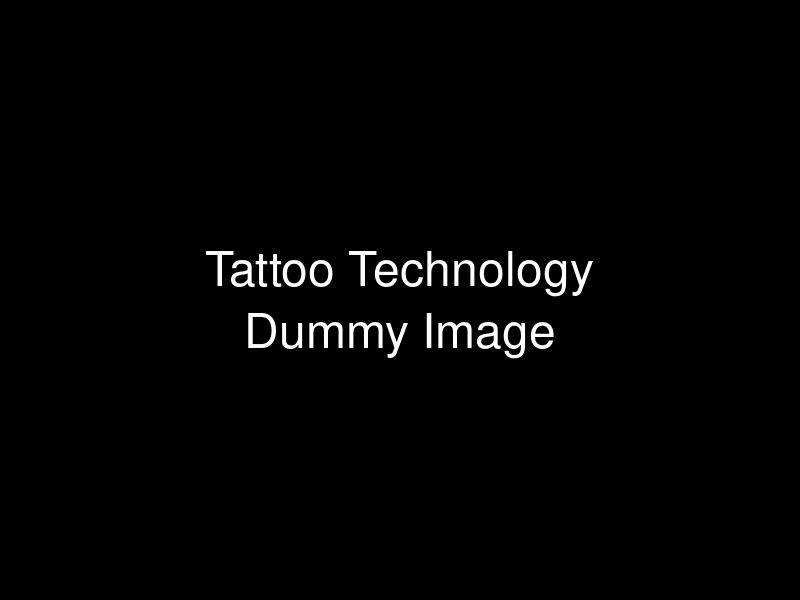
\includegraphics[width=0.8\textwidth]{figures/technology.png}
    \caption{A history of tattoos.}
    \label{fig:timeline}
\end{figure}

\subsection{Theory}

A tattoo $T = (s_1, s_2, \ldots, s_n)$ is a sequence of $n$ strokes $s_i$.
A stroke $s_i$ is sequence of needle poses $p_i$.
Each pose represents the position $\mathbf{p}_i \in \mathbb{R}^3$ and orientation quaternion $\mathbf{q}_i \in \mathbb{H}$.
The optimal angle of the needle is perpendicular to the skin surface.
We approximate this surface using a mesh $M_i$, which is a collection of vertices $V_i$, edges $E_i$, and faces $F_i$.
The arm is controlled in joint space $\mathbf{q} = (q_1, q_2, \ldots, q_j)$ where the number joints $J$ is $6$.
Inverse kinematics (IK) is the process that converts the joint space coordinates \( \mathbf{q} \) into the end effector space coordinates \( (\mathbf{p}_{ee}, \mathbf{q}_{ee}) \):
\[
\text{IK}: \mathbf{q} \mapsto (\mathbf{p}_{ee}, \mathbf{q}_{ee})
\]

\pagebreak

\section{tatbot}

\subsection{Hardware}

TatBot uses a pair of Trossen Robotics WidowXAI arms driven by dedicated controller boxes on a gigabit Ethernet network. The system employs a distributed computing architecture with multiple specialized nodes.

Perception is handled by two Intel RealSense D405 cameras---one mounted on the right arm and another mounted overhead---along with five Amcrest 5MP PoE turret cameras providing overhead coverage. The compute infrastructure includes an NVIDIA Jetson AGX Orin for AI inference, a System76 Meerkat PC for visualization and control, an Acer Nitro V 15 laptop for development, and two Raspberry Pi 5 computers for auxiliary tasks.

The tattoo application system consists of two Ambition Lutin rotary tattoo machines with 3.8mm straight drive bar stroke cams, powered by swappable 2200mAh RCA batteries operating at 5-12V with ±0.1V precision adjustment.

\begin{table}[h]
    \centering
    \caption{Compute and camera devices used by TatBot}
    \label{tab:hardware-devices}
    \begin{tabular}{lll}
        \toprule
        Device & Type & Specifications \\
        \midrule
        Jetson AGX Orin (\texttt{ojo}) & Compute & 12-core ARM Cortex-A78AE @ 2.2GHz, 32GB RAM, 200 TOPS \\
        Acer Nitro V 15 (\texttt{ook}) & Compute & Intel i7-13620H 16-core @ 3.6GHz, 16GB RAM, RTX 4050 6GB \\
        System76 Meerkat (\texttt{trossen-ai}) & Compute & Intel i5-1340P 16-core @ 4.6GHz, 15GB RAM \\
        Raspberry Pi~5 $\times$2 (\texttt{rpi1}, \texttt{rpi2}) & Compute & ARM Cortex-A76 4-core @ 2.4GHz, 8GB RAM each \\
        Intel RealSense D405 $\times$2 & Camera & 1280×720 RGBD, 90fps depth, USB3 connection \\
        Amcrest IP5M-T1179EW-AI-V3 $\times$5 & Camera & 5MP, 1920×1080, 5fps, 132° FOV, PoE \\
        \bottomrule
    \end{tabular}
\end{table}

\subsection{Software}

The TatBot system relies on a suite of open-source software packages organized into modular dependency groups:

\begin{itemize}
    \item \textbf{Core Dependencies:} The system uses \texttt{uv} for dependency management with Python 3.11.10. Core packages include \texttt{mcp} (v1.11.0) for Model Context Protocol communication, \texttt{paramiko} (v3.5.1) for SSH-based distributed computing, and \texttt{pyroki} for robotics kinematics and trajectory planning.
    
    \item \textbf{Robot Control (\texttt{bot}):} \texttt{lerobot} with TatBot-specific extensions for robot control, \texttt{trossen-arm} (v1.8.3) for WidowXAI arm interfacing, and \texttt{evdev} (v1.9.2) for input device handling.
    
    \item \textbf{Computer Vision (\texttt{cam}):} \texttt{opencv-python} (v4.11.0.86) for image processing, \texttt{pyrealsense2} (v2.55.1.6486) for Intel RealSense camera integration, and \texttt{pupil-apriltags} (v1.0.4.post11) for fiducial marker detection.
    
    \item \textbf{AI/ML Generation (\texttt{gen}):} \texttt{jax[cuda12]} (>=0.4.0,<0.5.0) for GPU-accelerated numerical computation, \texttt{jaxtyping} (>=0.2.25,<1.0.0) for JAX type annotations, and \texttt{jaxlie} (>=1.3.4,<2.0.0) for Lie theory operations in robotics.
    
    \item \textbf{3D Mapping (\texttt{map}):} \texttt{polyscope} (v2.4.0) for 3D geometry visualization, \texttt{potpourri3d} (v1.3.0) for 3D data processing, \texttt{trimesh} (v4.6.13) for mesh operations, and \texttt{pyglet} (v1.5.31) for OpenGL rendering.
    
    \item \textbf{Visualization (\texttt{viz}):} \texttt{viser} (v1.0.0) for 3D visualization and interactive browser-based GUIs, and \texttt{pyliblzfse} (>=0.4.1) for data compression.
    
    \item \textbf{Development (\texttt{dev}):} \texttt{isort} and \texttt{ruff} for code formatting and linting.
\end{itemize}

The system employs a distributed architecture with MCP servers running on individual nodes, enabling remote execution of tasks like camera calibration, skin scanning, and stroke visualization across the network.

\subsection{VLA}

Vision-Language-Action (VLA) models represent a new paradigm in robotics, enabling systems to interpret visual inputs, understand natural language instructions, and generate complex action sequences in the real world.
Recent advances such as $\pi$0 \cite{Black2024pi0}, GR00T N1 \cite{Bjorck2025gr00t}, and SmolVLA \cite{Shukor2025smolvla} have demonstrated the potential of large-scale, generalist VLA models to perform a wide range of tasks across diverse robotic platforms.
These models leverage massive datasets and transformer-based architectures to bridge the gap between perception, language, and control, paving the way for more flexible and capable autonomous agents.

\subsection{Data Recipe}

swiftsketch dataset - flux/ideogram/sdxl -> switftketch svg -> ply/mesh
meshformer dataset -

Vision Language Action (VLA) models are used to merge the semantic intelligence of large pretrained VLMs and fast robotic control performed with a Diffusion Model.
$\pi_0$ \cite{Black2024pi0}, GR00T N1 \cite{Bjorck2025gr00t}, and SmolVLA \cite{Shukor2025smolvla} have demonstrated the potential of large-scale, generalist VLA models to perform a wide range of tasks across diverse robotic platforms.


finetuned VLA with 
synthetic data generated heuristically from sim
real data from recorded tatbot sessions

huggingface for dataset management

there is a fundamental magic inside modern pretrained transformers.
The space of neural programs encoded in the weights just from human data on the internet is enormous. 
Some of these neural programs serve as useful starting points for robotic control.

\section{Results}

foo

\section{Discussion}

\subsection{Other Robotic Tattoo Systems}

Tattoos are fundamentally 3D.
They flow over the surfaces and curves of the body.
Every single previous robotic tattoo system has been constrained to the 2D plane.
Robot arms have been used before, but the control is still classical.
A set of waypoints are programmed by the human operator and the robot arm just simply executes.
Modern attempts have focused on 2D gantry systems, similar to 3D printers.
Even the designs are not AI generated, but rather come from a library of pre-existing human designs.
These robots are not artists, they are printers.
Technology has advanced and we need to create new systems that go beyond these limitations.
AI generated designs that are 3D by nature tattooed using a robotic arm controlled by AI.
Using modern imitation learning and reinforcement learning.

foo \cite{NietoBastida2023}
foo \cite{arar2025swiftsketch}
foo \cite{carlier2020deepsvg}
foo \cite{mellor2020unsupervised}
foo \cite{ha2017neural}
foo \cite{huang2019learning}
foo \cite{kotani2019teaching}

Various tattoo robots based on modified 3D printers have been demonstrated on YouTube \cite{EmilyTheEngineer2025}, a similar system \cite{YamanDeif2021}

\subsection{Robotic Artistry}

technology can create social tensions.
photography was frowned upon by those who feared it would replace portraiture.
robotic tattooing will run into tensions with human tattoo artists.
new art mediums do not replace old art mediums, they simply expand the canvas with which humanity can express itself.

\subsection{Future Work}

As it stands, tatbot is still just a proof of concept.
The design space is limited, the accuracy is still suboptimal.
My dream is to continue to work on this project, expanding it accross the world.
Cities are the heart of tattoing, where a large population creates an endless supply of skin.

\section{Conclusion}

foo

\bibliographystyle{plain}
\bibliography{references}

\end{document} 